\section{Performances} % (fold)
\label{sec:perf}

Pour les performances, nous avons créé un script qui nous permet de lancer des jobs sur la machine Plafrim de l'Inria et de tracer le graphique associé directement. Par défaut le mot de passe à trouver est \emph{passwd}, avec comme alphabet les $26$ lettres minuscules. Le programme est lancé sur un nombre grandissant de processus -- de $2$ à $32$ mais pas forcément par incrément de $1$ -- et une moyenne est faite sur $5$ exécutions. Un exemple de sortie est le graphe de la figure \ref{fig:graph_procs} sur lequel nous pouvons constater une très forte accélération à partir de $3$  et $4$ processus. Le fait que la courbe reste constante par la suite est du au surcoût de communication qu'engendre le programme avec trop de processus. Nous avons essayé de relancer la création du graphe pour le mots de passe $passwrd$ mais la première itération avec un seul esclave prend trop de temps.

\begin{figure}[h!]
\centering
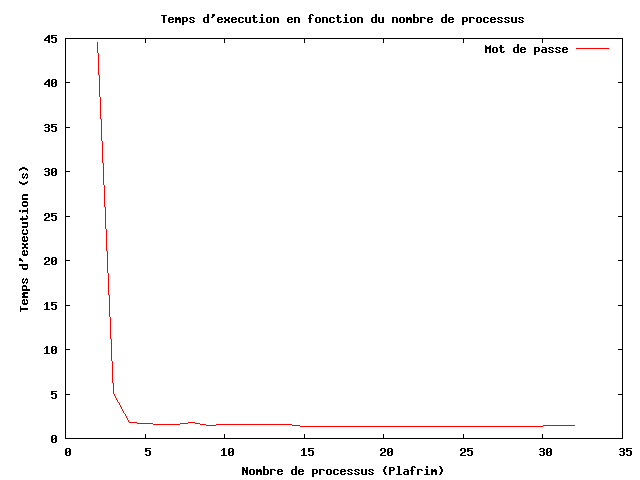
\includegraphics[width=0.8\textwidth]{1_graph_procs}
\caption{Résultats obtenus sur Plafrim}
\label{fig:graph_procs}
\end{figure}

